\section{Methodology}
\subsection{Node Design and Functionality}


Each node follows the basic rules of gossip. That is, on every round a node will gossip to itself with probability ½ or with any one of its neighbors with probability $1/(\textrm{Number of neighbors} * 2)$. Our implementation conducts both push and pull once per gossip round. In addition to the push and pull cycle, each node will simultaneously update its local values. Unlike most example implementations, our nodes conduct all calculations simultaneously.
Nodes are first initialized with a fragment of any size. Upon initialization, the node runs local calculations for minimum, maximum, average, and median values. Once this is complete, the node will also replicate its fragment to its neighbors. All nodes are responsible for a single fragment, but may store any number of fragments as replicas or while passing fragments over the network. When a node receives a new fragment to own, it will reinitialize itself and replicate the new fragment. It is important to note that since each node is responsible for a single fragment, the fragment’s “number” is synonymous with the process ID of it’s owner node. We do tend to map actual numbers on top of the node process IDs, but this is as a matter of convenience.

Once a node is done with its initialization, it is ready to gossip. Our implementation requires all nodes to wait for a “step” signal to be sent before executing each round. This allows us to precisely measure the number of rounds executed and gives us excellent control over the network as a whole.

On each gossip round, all nodes push and pull their local values with their neighbors. Once a node receives new data for any calculation (remember, we do all calculations simultaneously), it will update its local data according to the data received.

For calculating the minimum and maximum values, a simple min/max comparison of the node’s current value with the received value is sufficient. Calculating the average is similarly trivial as it is a well documented process of dividing the sum of the current and new average values by two.

[Insert min, max, and average formulas here in latex]
\begin{equation}
Avg(x_i)=\frac{x_i + x_j}{2}
\end{equation}


Calculating the median can be approached from many angles. Attempting to find the “median of medians” by recording each median value received was considered. However, this approach essentially requires a node to have knowledge of global state. Recording the most frequent numbers and finding their median was also considered, but again it would be vastly skewed over the whole of the network. Finally, a method similar to averaging was used, where the current median is added to the new median and the sum is divided by two. This was motivated by the method for finding the median in a set of even size.

[Insert formula for median here in latex]

Fragment handling is best examined in two phases. First, each node is the owner of but one fragment. The node will use its fragment for initialization as discussed, but after this is done the node’s duty becomes serving up and updating the fragment. When a node receives a request to store a fragment, it first checks to see if it is the owner of the fragment by looking at the PID assigned to be the owner of the fragment. Remember, our implementation uses PIDs as the actual fragment numbers. If the node owns the fragment, it will replace its current fragment with the new one and reinitialize itself. If a node does not own the fragment it will gossip the fragment along.

When a request for a fragment is issued the following occurs. First, the node checks the request to see if it has the requested fragment. If it doesn’t, the node will change the sender field of the request to its own PID and gossip the request on. If it does have the fragment, the node will send it back to the sender of the request. Note that this may not be the originator of the request. When a node issues a request, it sets a special field that indicates which node issued the request. This field does not affect the transmission directly, rather it allows a node to see if the reply is intended for it. If a node gets a reply that is intended for it then it will store the fragment, otherwise it will gossip the fragment reply on.

The second phase of fragment handling is replication. When a node receives a fragment to own, the node will replicate the fragment to its neighbors. Each node then maintains a list of fragments in addition to the fragment it owns. For example, if all nodes have three neighbors, all the nodes will actually hold four fragments – its own plus the replicas of the three neighbors.

This adds a layer of complexity to fragment stores and requests. The protocol described above still is in full effect, but with a couple of extra steps. When a node receives a request to store a fragment, it not only checks that it is the owner of the fragment, but that it has a replica of the fragment. If it has a replica of the fragment, it will update its own copy and then gossip the request along. If a node receives a request for a fragment, the node will again check to see if it has a replica. If there is a replica it will send the replica as a response.

Looking at this as a whole then, we have a system that provides a gossip-based read one, write all functionality. When writing, all nodes with a copy of the fragment are updated either directly or by the replication function of the owner node. When reading, any one of the nodes containing the fragment – either owning it or replicating it – will respond with the fragment.

\subsection{Network Design}
The network is constructed as two trees, joined at the leafs. This joint between the trees is the bisection of the network. Starting from the root node in each tree, each node has two children. We build the trees in breadth first order to a maximum depth. For simplicity, we restrict ourself to having the same number of nodes in each tree and ensure that the trees are balanced. The trees are stored in Erlang’s digraph data structure. We tried have our network have the same properties as discussed in GOSSIP analysis. Our network is undirected and not regular (some nodes have degree 2, most have 3). In real world applications, sensor networks can be sparse. Our network reflects that characteristic. It is irreducible, that is there exist paths
from every node to any other nodes. Also, nodes can talk to themselves which makes the network aperiodic and subsequently the transition probability matrix of our network is right stochastic since not all nodes have the same degree.

\begin{figure}[ht!]
\centering
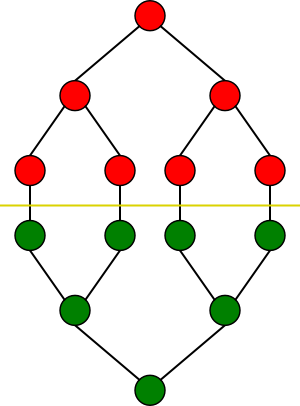
\includegraphics[width=90mm]{network.png}
\caption{Small scale example of our network. Yellow line is the network bisection.}
\label{overflow}
\end{figure}

Our network is not double stochastic, which will affect its conductance. The conductance will not be as high as a regular graphs, but will be good enough for our experiment. We still expect convergence to happen. We research matrix normalization techniques such as Richard Sinkhorn’s theorem for making a matrix for finding a doubly stochastic matrix from a square matrix and diagonal matrices, but chose not to implement it in our design.
Network construction was implemented in a library. First the user supplies a number of desired nodes and gets back the number of nodes in the network. With this information, the user spawns that number of nodes and records their PIDs in a list. Finally, the user supplies this list to a function that creates the digraphs and joins them, returning to the user a final digraph. A few helper methods are also present in this library. The most important is the get\_neighbor methods. The user can supply the digraph of the network and a PID and return get a list of the neighbors of this node. 

\subsection{Convergence}
Convergence
Our network does not exhibit properties that make an analysis easy. We have to remember the fact that in using gossip we trade accuracy for latency. Therefore, we chose not to do an extensive analysis and instead focus on experimental measurements. We were interested in experimentally determining two qualities. First, we wanted to study how the size of the network and the nature of the computation affects the time to converge on an answer. Second, we wanted to figure out how the size of the network and the computation affect the error over time. Since we could not compute the error during the design of the system, we chose an acceptable point of convergence of when the error was less than or equal to 3\%. 
